

%%% This LaTeX source document can be used as the basis for your technical
%%% report. Intentionally stripped and simplified
%%% and commands should be adjusted for your particular paper - title, 
%%% author, citations, equations, etc.
% % Citations/references are in report.bib 

\documentclass[conference,backref=page]{acmsiggraph}
\usepackage{listings}
\usepackage[]{algorithm2e}
\TOGonlineid{45678}
\TOGvolume{0}
\TOGnumber{0}
\TOGarticleDOI{1111111.2222222}
\TOGprojectURL{}
\TOGvideoURL{}
\TOGdataURL{}
\TOGcodeURL{}

% Include this so that citations show up in blue and the page information is included in the reference section
\hypersetup{
    colorlinks = true, 
    linkcolor = blue,
    anchorcolor = red,
    citecolor = blue, 
    filecolor = red, 
}


\title{Model shattering using real-time collisions\\
	   Final Report}

\author{Conner Weatherston \thanks{e-mail:40167111@live.napier.ac.uk} \\
Edinburgh Napier University\\
Physics-Based Animation (SET09119)}
\pdfauthor{Conner Weatherston}

\keywords{Rigid body, collision detection, bounding volumes, mesh destruction, OpenGL, real-time, physics, computer graphics, optimisation}

\begin{document}

\teaser{
   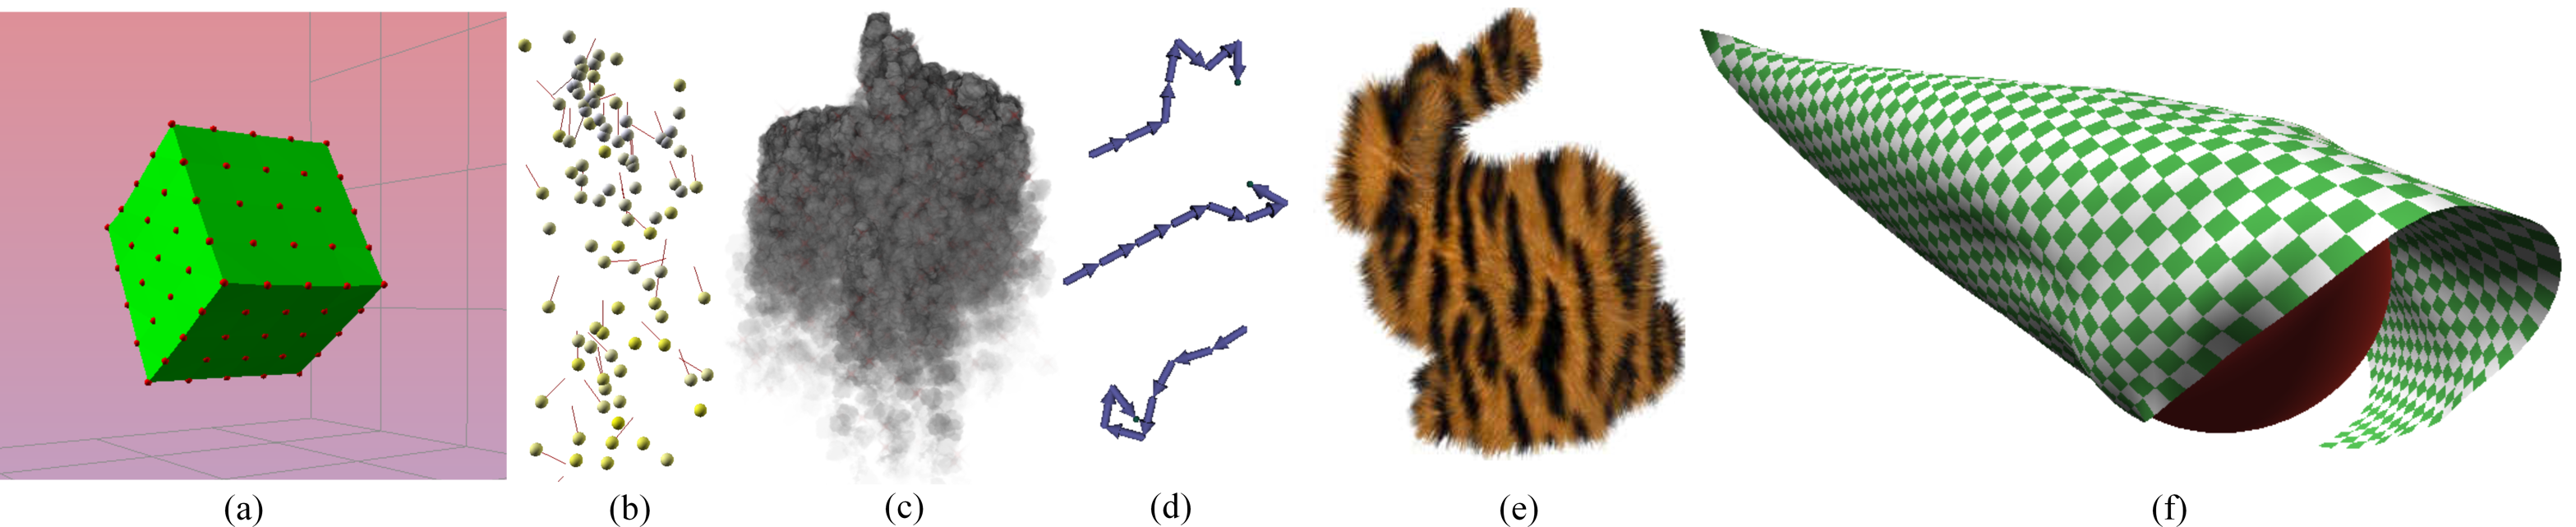
\includegraphics[height=1.5in]{images/sampleteaser}
   \caption{(a) mesh slicing, (b) collision response, (c) collisions resting on colliders}
   \label{fig:teaser}
 }

\maketitle

\raggedbottom

\begin{abstract}
In most physics based games, destructible objects are typically loaded in with their shattered fragments on run-time. This means that sometimes the fracture look unnatural. The aim of this physics simulation is hoping to look at is ways to slice meshes in real time to generate new fragments.

The approach looked at the in the design report suggested a technique called voronoi shattering \cite{voronoishattering} in order to break the objects up into random fragments. However this was not implemented in the final simulation due to difficulty of producing 'Delaney Triangulation' and time constraints. Therefore a simpler approach was used where the object is split recursively using a series of random planes which intersect through the model mesh. Each fragment produced would have one less splitting plane, thus putting a cap on how far a model can fracture.

\end{abstract}

\keywordlist

\section{Introduction}

In most video games, destructible objects are pre-computed models which are the equivalent of the model fragments. The purpose of this simulation is to create proper mesh fragments in real-time just using the original meshes information. A key part of this simulation is optimisation as creating new objects is an expensive process.

\section{Related Work}

Currently there are several plugins that use either the same idea or has a similar solution. However these are mostly implemented into modelling software where optimisation is not an issue as it is not required in a real-time environment. The tutorial provided by \cite{voronoiShattering} helped to provide a solution on slicing meshes using planes. \cite{Physics} bullet physics library provided help in creating the physics for this simulation. 

\section{Simulation}

\paragraph{Overview} \hfill

The simulation is revolved around having objects in a real-time environment interact with each other. In this simulation, the objects have been kept to cube or cuboid shapes for simplicity. There is also a plane which acts as the 'floor' of the scene. When objects collide with each other they respond in a realistic manner. In order for a collision to cause an object to break a certain threshold must be reached. If this limit is reached for the object then it will split apart depending on its splitting planes, which determine how the model will shatter. Another condition is also in place to determine if both or one of the models will shatter.

\paragraph{Implementation} \hfill

The implementation of this project can be broken down into three major parts. Rigid bodies, collisions and meshes.

\paragraph {Collision detection} \hfill

It is incredibly inefficient to test meshes directly against each other as this would require testing each vertex of object A against every vertex in object B. Therefore bounding volumes are required which provide simpler tests that are not as costly in performance. The downside to this is the response may not be accurate when a collision is detected depending on what collider approach is used. In this simulation three types of colliders have been utilised. These are the plane collider, the sphere collider and the orientated bounding box (shortened to OBB). 

As this simulation is focused on cubes the most suitable collider is the OBB as it fits well with the objects. However a sphere collider is attached in order to improve performance. Instead of testing for an OBB to OBB collision each tick, it is cheaper and faster to check two sphere colliders, thus if two sphere colliders are in contact then an OBB OBB intersection check shall be performed. 


\cite{BoundingVolume} Provided a good starting place to find information on each of the colliders and how the intersections tests between them should be done.

\subparagraph{Collider} \hfill

This is an abstract class which all colliders will inherit from. As every collider requires a position and an update method it has been initialised here.

\begin{lstlisting}
abstract Class Collider
{
	Vec3 position;
	double radius;
	// This is used to update
	// the position of the colliders.
	virtual void Update(double deltaTime); 
}
\end{lstlisting}

\subparagraph{Plane collider} \hfill

The plane collider is used to simulate the floor. However as the floor is not meant to have true rigid body properties. i.e it should not 'fall' as it will never move, therefore there is a plane collider and a graphic drawn for it rather than being a true 'Model' object in the scene.

\begin{lstlisting}
Class PlaneCollider : public Collider
{
	Vec3 normal;
}
\end{lstlisting}

\subparagraph{Sphere collider}  \hfill 

The base class is esentially a sphere collider, as it has all the same propierties, therefore the sphereCollider inherits from the collider class, this is because the Collider class is abstract so it cannot be used directly.
\begin{lstlisting}
Class SphereCollider : public Collider
{
	void Update(Vec3 newPosition) { SetPosition(newPosition);  }
}
\end{lstlisting}

\subparagraph{Orientated bounding box}\hfill 

This is a stage further in complexity to an axis aligned box, however it can handle rotations. As there are more checks that a required for an OBB to OBB intersection it is important to only check when it is necessary to, and not every tick. In order to create an OBB the corners are required. To reduce the memory required to store an OBB, only two opposite corners are stored, as the other corners can be produced using a combination of these two corners.

\begin{lstlisting}
Class BoundingBox : public Collider
{
	double topX,topY,topZ;
	double botX,botY,botZ;
	quat rotation;
	
	void Update(RigidBody body) {rotation = body.orientation; SetPosition(body.position);}
	
}
\end{lstlisting}

The rotation of the box is done in the intersection check. The rotation is taking from the orientation of the rigid body. This will ensure that the object stays inside the bounding volume.

The corners are calculated from a model mesh. It takes all the vertex corners and looks for the extreme values on each axis in order to produce a box that will encompass the model.

\subparagraph{Intersection detection} \hfill

Each physic tick a intersection test stage is required to find if there is collision between models. 
There are several possible detections used in this simulation. There is:
\begin{itemize}
	\item Sphere - Sphere
	\item Sphere - Plane
	\item Box - Plane
	\item Box - Box.
\end{itemize}

The sphere detection is used to calculate when an object is almost in collision range. This is used to optimise the code as it prevents expensive box calculations from being computer each tick, until objects are close enough.

\begin{algorithm}
	\KwData{Sphere collider A, Sphere collider B}
	\KwResult{Boolean}
	distance = length(B.position- A.position); \hfill
	
	sumRadius = A.radius + B.radius;\hfill
	
	\If{(distance $<$ sumRadius)}
	{	
		return true;
	}
	return false;
	\caption{Sphere - Sphere detection}
\end{algorithm}

\begin{algorithm}
	\KwData{Sphere collider A, Plane collider P}
	\KwResult{Boolean}
	Vec3 tempVec = A.position - P.position;
	double distance = dot(tempVec,P.normal);
	\If{(distance <= A.radius)}
	{
		return true;
	}
	return false;
	\caption{Sphere - Plane detection}
\end{algorithm}

\begin{algorithm}
	\KwData{Bounding Box A, Plane collider P}
	\KwResult{Boolean}
	\For{each corner in A}
	{
		distance = dot(p.position, P.normal) - dot(corner, p.normal);
		\If{(distance > 0)}
		{
			return true;
		}
	}
	return false;
	
	
	\caption{Box - Plane detection}
\end{algorithm}

\begin{algorithm}
	\KwData{Bounding Box A, Bounding Box B}
	\KwResult{Boolean}
	\For{each corner in A}
	{
		\If{(corner in max/ min x range of B)}
		{
			\If{(corner in max/ min y range of B)}
			{
				\If{(corner in max/ min z range of B)}
				{
					return true;	
				}	
			}
		}
	}
	return false;
	
	\caption{Box - Box detection}
\end{algorithm}


\paragraph{Rigid bodies} \hfill

In order to have a simulation which simulates proper physics, rigid bodies need to be attached to the objects. An rigid body consists of the following: position, previous position, mass, inverse mass, orientation, forces being applied to the object. 
\begin{lstlisting}
Struct RigidBody
{
	double mass;
	double inverseMass;
	dvec3 position;
	dvec3 previousPosition;
	dvec3 forces;
	dvec3 torques;
	dquat orientation;
}

\end{lstlisting}

\paragraph{Meshes} \hfill

The mesh information needs to be stored and cannot be put straight onto the OpenGL buffers. This is because the data cannot be accessed and used to split the geometry. Therefore , the information is stored in a 'ModelInfo' struct, which holds the geometries vertex position, texture coordinates, normals and colours.
 
In order to split a mesh a splitting hyperplane is required. This plane separates the geometry into two segments, One which is the 'new' fragment and the other is the new updated original model which has been fractured. 

Triangle is a class that has been created that will store 3 vertices (in the correct order) that represents a triangle that is rendered on the polygon.

\begin{algorithm}
\KwData{Model to be split, plane to split by}
\KwResult{New Model}
Vector$<$Vec3$>$ fragment vertices.  \hfill

\For{each Triangle in ModelInfo positions}
{
		Integer pointsInfront = 0; \hfill 
		\For{each point in Triangle}
		{
			\If{dot(TrianglePoint, planeNormal)
			 - dot(planePoint,planePoint) $>$ 0} 			 
			{
				pointsInfront++;
			}
		}
	\If{pointsInfront == 3}
	{
		push triangle points to fragment vertices;
	}
	\If{points == 0}
	{
		push closest points to plane to fragment vertices;
	}
		\For{(each point in Triangle)}
		{
			\If{dot(TrianglePoint, planeNormal)
				- dot(planePoint,planePoint) $>$ 0} 			 
			{
				add point to fragment vertices; 
			}	
			\Else
			{
				push closest point to plane to fragment vertices;
			}
		}
	}
 \caption{New fragment creation}
\end{algorithm}

The algorithm is reversed to find the vertices of the updated model. Essentially where there is a $>$ replace it with a $<$ and vice versa.






\paragraph{Update} \hfill

To create an realistic simulation a concept of a 'physics tick' is required. This is in place in order to decouple the physics from the frame-rate. Thus the physics will run the same if the frame rate is at 10 FPS or 60 FPS.  

There are three parts to the physics update. There are summarised below:

\subparagraph{Colliding object}
The first stage is detecting if any objects are currently colliding with each other.
If there is a collision between two objects then a struct called 'CollisionInfo' is created which contains the following data:

\begin{itemize}
\item{Pointer to object A.}
\item{Pointer to object B.}
\item{Depth of overlap in objects.}
\item{Direction to be pushed towards.}
\item{Position of collision.}
\end{itemize}

This struct is then pushed back onto a vector; which contains all the collisions that have happened between the models in this current update.
\subparagraph{Resolve collisions}\hfill

For each of the collisions that have occurred a resolve stage needs to occur. This calculates what should happen to each object in terms of direction it is now going; the velocity of the objects and if the proper conditions have been met, zero, one or both objects shatter.
\subparagraph{Integrate rigid bodies}\hfill

After collisions have been sorted, each model need to update their current position, previous position, orientation. This is done by a form of Euler integration as this is an impulsed based physics simulation.

% EVALUATION
\section{Testing and evaluation}

In order to test the splitting a meshes in this simulation a series of hard coded planes were tested against. The results were already known thus is was just a simple comparison between the expected results and the actual results. If there was a discrepancy then there was an issue with mesh cutting algorithm. The first error was noticed when the split was done in the proper shape however some of the triangles were missing from the polygon. This was because the ray cast approach to find the point of intersection would lead to faces on the model missing. This would have been rectified by triangulating the model. However An easier solution was the one presented earlier; where finding the closest point to the plane proved not only simpler, but more accurate as well.

The collisions were done in two stages. The first stage was testing that the colliders recognised that they were in contact with each other. This was tested by having a message print to console when two colliders contacted and the message specified which colliders were in contact. 

The following stage, which was resolving collisions, was more difficult. The only way to test if the algorithm put in place worked properly was to run it several times and used different conditions to ensure that the colliders responded in a sensible manner. What was noticed from this was an OBB collider had issues sitting on other objects. If it was ontop of a plane collider it would keep rotating, If it was on top of another OBB collider it would sink into the object before coming back out and starting jumping on top of it. Due to time restraints a proper solution to this was not implemented. So the resolution uses simple sphere resolution as this provides a decent solution.



\section{Conclusion and Future work}

Future work on this project can be undertaken. The next step would be creating convex shapes instead of just cubes and cuboid, once this has successfully undertaken then it would be possible to undertake the voronoi shattering technique that was originally suggested as this would provide the planes that the model would be split by. Also filling the model in order to fix missing/ incorrect faces would be a reasonable step forward. This would improve the visual look of this project at the cost of performance as it take longer to fix the model.


% \section*{Acknowledgements}


\bibliographystyle{acmsiggraph}
\bibliography{report}

\end{document}

